\documentclass[a4paper]{article}

\usepackage[english]{babel}
\usepackage[]{algorithm2e}
\usepackage{algorithm}
\usepackage[utf8x]{inputenc}
\usepackage{amsmath}
\usepackage{graphicx}
\usepackage[colorinlistoftodos]{todonotes}
\title{Joint Modeling of Content-Partitioned Multinetwork Embeddings (CPME) and Point Process Approach}
\author{Bomin Kim}

\begin{document}
\maketitle

\begin{abstract}
Your abstract.
\end{abstract}

\section{Ideas}
Current CPME model does not involve any of temporal component, which plays a key role in email interactions. Intuitively, past interaction behaviors significantly influence future ones; for example, if an actor $i$ sent an email to actor $j$, then $j$ is highly likely to send an email back to $i$ as a response (i.e. reciprocity). Moreover, the recency and frequency of past interactions can also be considered to effectively predict future interactions. Thus, as an exploratory data analysis, point process model for directional interaction is applied to the North Carolina email data. Starting from the existing framework focused on the analysis of content-partitioned subnetworks, I would suggest an extended approach to analyze the data using the timestamps in the email, aiming to develop a joint dynamic or longitudinal model of text-valued ties.\\ \newline
 CPME model is a Bayesian framework using two well-known methods: Latent Dirichlet Allocation (LDA) and Latent Space Model (LSM). Basically, existence of edge depends on topic assignment t (LDA) and its corresponding interaction pattern c. Each topic t=1,…,T has one interaction pattern c=1,…,C, and each interaction pattern posits unique latent space (LSM), thus generating $A\times A$ matrix of probabilities $P^{(c)}$ that a message author
a will include recipient $r$ on the message, given that it is about
a topic in cluster $c$.  Incorporating point process approach, now assume that under each interaction pattern, we have $A\times A$ matrix of stochastic intensities $\lambda^{(c)}(t)$ which depend on the history of interaction between the sender and receiver. 
\newpage
\section{CPME + Point Process Model}
Before we build up the ultimate joint model of LDA, LSM, and point process approach, we first start with simpler model which combines LDA and point process approach.
\subsection{Generative Process (From Mattew Denny)}
First we generate the global (corpus-wide) variables. There are two main sets of global variables: those that describe the
topics people talk about and those that describe how people interact (interaction patterns). These variables are linked by a
third set of variables that associate each topic with the pattern that best describes how people interact when talking about
that topic. There are T topics. Each topic $\phi^{(t)}$ is a discrete distribution over V word types \textbf{[See Algorithm 1].} There are C
interaction patterns. \\ \newline \textcolor{red}{1) Univariate Hawkes approach:} Each interaction pattern consists of a A-dimensional vector of stochastic intensity $\lambda^{(c)}(t)$ that model the rate at which each sender $a$ sends email at time $t$ given all messages received by $a$ at times
$r_k^{a}< t$ ($r_k^{a}$ is the timestamp of $k^{th}$ email received by $a$)  \textbf{[See Algorithm 2].}  \\ \newline
 \textcolor{red}{2) Multivariate Hawkes approach:} Each interaction pattern consists of a A$\times$A matrix of stochastic intensity $\lambda^{(c)}(t)$ that model the rate at which each sender $a$ sends email to actor $r$ at time $t$ given all messages received by $a$ from $r$ at times
 	$r_k^{ar}< t$ ($r_k^{ar}$ is the timestamp of $k^{th}$ email received by $a$ from $r$)  \textbf{[See Algorithm 3].}  \\\newline  (Later goal: We also associate each sender–recipient pair with an observed P-dimensional
vector of covariates $x^{(ar)}$; however, we assume that our generative process is ocnditioned on these covariates.)  The topics and interaction patterns are tied together via a set of T categorical variables (one per topic). These variables
associate each topic with a single interaction pattern \textbf{[See Algorithm 4].} Then, we generate the local variables. There are D
emails. We assume that each email’s sender $a^{(d)}\in [A]$, timestamp $t^{(d)} \in [0, T]$, and length $N^{(d)} \in N_0$ are observed; we do not generate these variables  \textbf{[See Algorithm 5].}
 \begin{algorithm}[H]
 	\SetAlgoLined
	\caption{Topic Word Dstributions}
	\For{t=1 to T}{
		draw $\phi^{(t)}$ $\sim$ Dir($\beta, \bf n$)
}
\end{algorithm}
\begin{algorithm}[H]
	\SetAlgoLined
	\caption{Interaction Patterns using univariate Hawkes Process}
	\For{c=1 to C}{
		\For{a=1 to A}{
			set $\lambda_a^{(c)}(t)=\mu_{a}+\theta_{a}\sum\limits_{r_k^{a}< t}g_a(t-r_k^{a}) \quad (=\mu_{a}+\theta_{a}\sum\limits_{r_k^{a}< t}w_{a} e^{-w_a(t-r_k^{a})})$
			
			Note: In the context of e-mails, the background rate $\mu_a$ can be interpreted as that rate at
			which actor $a$ sends email that are not replies to emails received from other actors. In other words, $\mu_a$ is the baseline rate at which $a$ initiates new email threads.
			Each message received by actor $a$ at time $r_k^{a}$
			elevates the overall rate of sending
			emails at time $t >r_k^{a}$
			, through the triggering function, which is assumed
			to be exponential. $\theta_a$ can be interpreted as the reply rate for actor $a$, since it is the total expected number of replies, on average, sent by actor $a$ per email received from another actor in the network. The speed at
which actor $a$ replies to emails is governed by the parameter $w_a$, with larger values of
$w_a$ indicating faster response times for actor $a$. Indeed, ${w_a}^{-1}$ is the expected number of hours it takes for actor $a$ to reply to a typical email.}
} 
\end{algorithm}
\begin{algorithm}[H]
		\SetAlgoLined
	\caption{Interaction Patterns using multidimensional Hawkes Process}
	\For{c=1 to C}{
			\For{a=1 to A}{
	set $\lambda_a^{(c)}(t)$ as the A-dimensional vector of rates defined by a point process $N_t^a$.\\
		\For{r=1 to A}{$\lambda_{ar}^{(c)}(t)=\mu_{ar}+\theta_{ar}\sum\limits_{r_k^{ar}< t}g_{ar}(t-r_k^{ar}) (=\mu_{ar}+\theta_{ar}\sum\limits_{r_k^{ar}< t}w_{ar} e^{-w_a(t-r_k^{ar})})$

	Note: In the context of e-mails, the background rate $\mu_{ar}$ can be interpreted as that rate at
which actor $a$ sends email that are not replies to emails received from actor $r$. In other words, $\mu_{ar}$ is the baseline rate at which $a$ initiates new email threads to $r$.
Each message received by actor $a$ from actor $r$ at time $r_k^{ar}$
elevates the overall rate of sending
emails at time $t >r_k^{ar}$
, through the triggering function, which is assumed
to be exponential. $\theta_{ar}$ can be interpreted as the reply rate for actor $a$ to actor $r$, since it is the total expected number of replies, on average, sent by actor $a$ per email received from actor $r$ in the network. The speed at
which actor $a$ replies to actor $r$ is governed by the parameter $w_{ar}$, with larger values of $w_{ar}$ indicating faster response times for actor $a$ to actor $r$. Indeed, ${w_{ar}}^{-1}$ is the expected number of hours it takes for actor $a$ to reply to actor $r$ a typical email.}}}
\end{algorithm}
\begin{algorithm}[H]
		\SetAlgoLined
	\caption{Topic-Interaction Pattern Assginments}
	\For{t=1 to T}{
		draw $l_t$ $\sim$ Unif(1, C)
	}
\end{algorithm}
\begin{algorithm}[H]
	\SetAlgoLined
	\caption{Topic-Interaction Pattern Assginments}
	\For{t=1 to T}{
		draw $l_t$ $\sim$ Unif(1, C)
	}
\end{algorithm}
\section{Preliminary Analysis}
Hurricane Sandy was the most destructive hurricane in 2012, which hit North Carolina on late October (October 28, Governor Bev Perdue declared a state of emergency in 24 western counties due to snow and strong winds). In our dataset, there are three counties which cover the date of Hurricane Sandy (October 22, 2012 – November 2, 2012), so we focus on the three counties, since the timestamp of email in this case is much more important than usual case without any disastrous event.
\subsection{Dare County}
\footnotesize
\begin{table}[ht]
	\centering
	\begin{tabular}{ |c|ccc|c| } 
		\hline 
		\textbf{Period} &\textbf{Before Sandy} & \textbf{During Sandy} & \textbf{After Sandy} & \textbf{Overall} \\ 	\hline
			\textbf{\# emails}& 1933 & 1563 & 1467 & 4963 \\ 
		\hline
	\end{tabular}
	\caption{ Summary of Dare county email data based on time period}
	\label{table:nullDare2}
\end{table}
\normalsize
Before Sandy ranges from 2012-09-01 to 2012-10-21 (7 weeks), During Sandy ranges from 2012-10-22 to 2012-11-02 (2 weeks), and After Sandy ranges from 2012-11-03 to 2012-11-30 (4 weeks).
\footnotesize
\begin{figure}[ht]
	\centering
	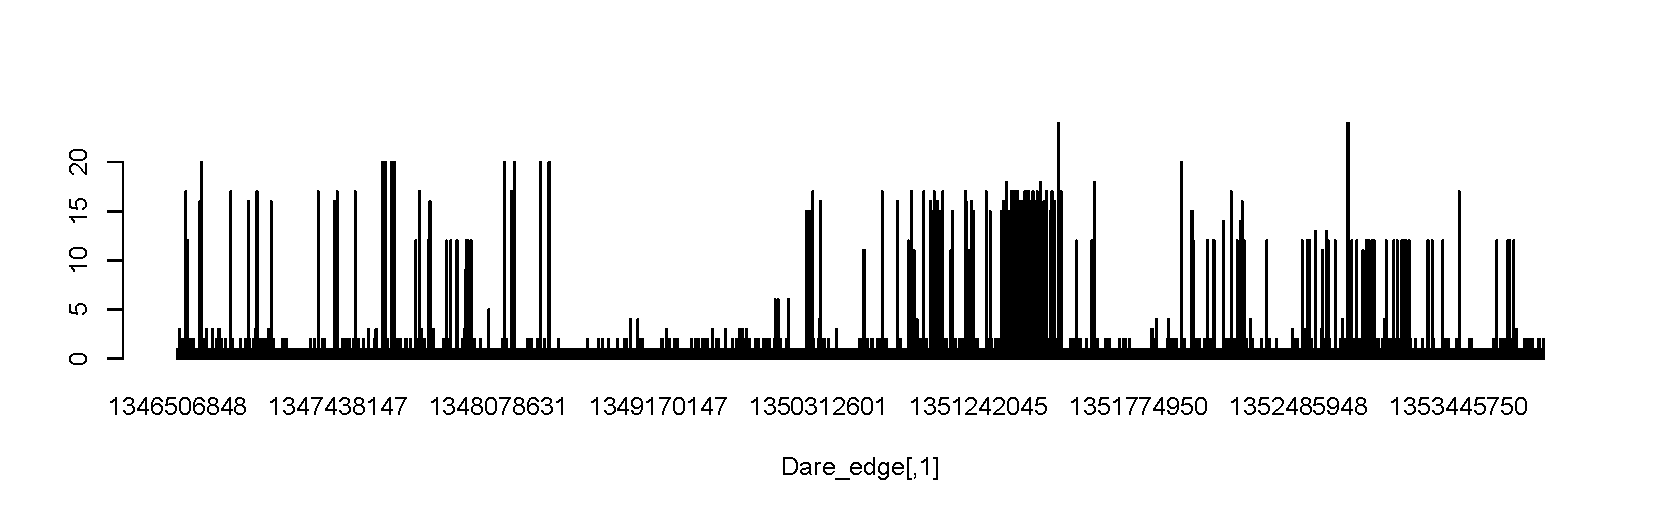
\includegraphics[width=1.1\textwidth]{DareEmails.pdf} 
	\caption{Frequency of Dare county emails from 2012-09-01 to 2012-11-30  }
	\label{fig:Emailplots}
\end{figure}
\begin{table}[ht]
	\centering
	\begin{tabular}{ |c|cc| } 
		\hline 
		\textbf{Time Interval} &\textbf{send} & \textbf{receive} \\ 	
		\hline  $[-\infty, t)$&  2.128, 2.659, 2.355, 2.919& 0.292, 0.257, 0.047, 0.110\\  $[t-30 m, t)$ &  0.262, -0.064, 0.782, 0.317 &2.087, 1.287 , 2.346, 1.870\\  $[t-2h, t-30m)$& 0.383, 0.157 , 0.024, -0.045 &0.553, 0.082, 0.794, 0.269\\ $[t-8h, t-2h)$ & 0.816, 0.054 , 0.077, 0.381 &-0.221, 0.048, 0.298, -0.012 \\ $[t-32h, t-8h)$& 0.085, 0.014,  0.228, 0.070 &0.101, 0.017, -0.033, 0.019\\ $[t-5.33d, t-32h)$&  0.103, 0.025, 0.092, 0.008 &-0.027, -0.016, -0.033, -0.009 \\ $[t-21.33d, t-5.33d)$  & 0.052, 0.000, 0.059, 0.010& 0.013, 0.030 , -0.016, 0.013\\ 
		$[-\infty, t-21.33d)$  & 0.052, 0.103, 0.027, 0.021  & 0.008, 0.000, 0.020, -0.005\\
		\hline
	\end{tabular}
	\caption {Estimated coefficients and approximate standard errors for dyadic effects of Dare county data (before Sandy, during Sandy, after Sandy, overall)}
	\label{table:nullDare}
\end{table}
\footnotesize
\begin{figure}[ht]
	\centering
	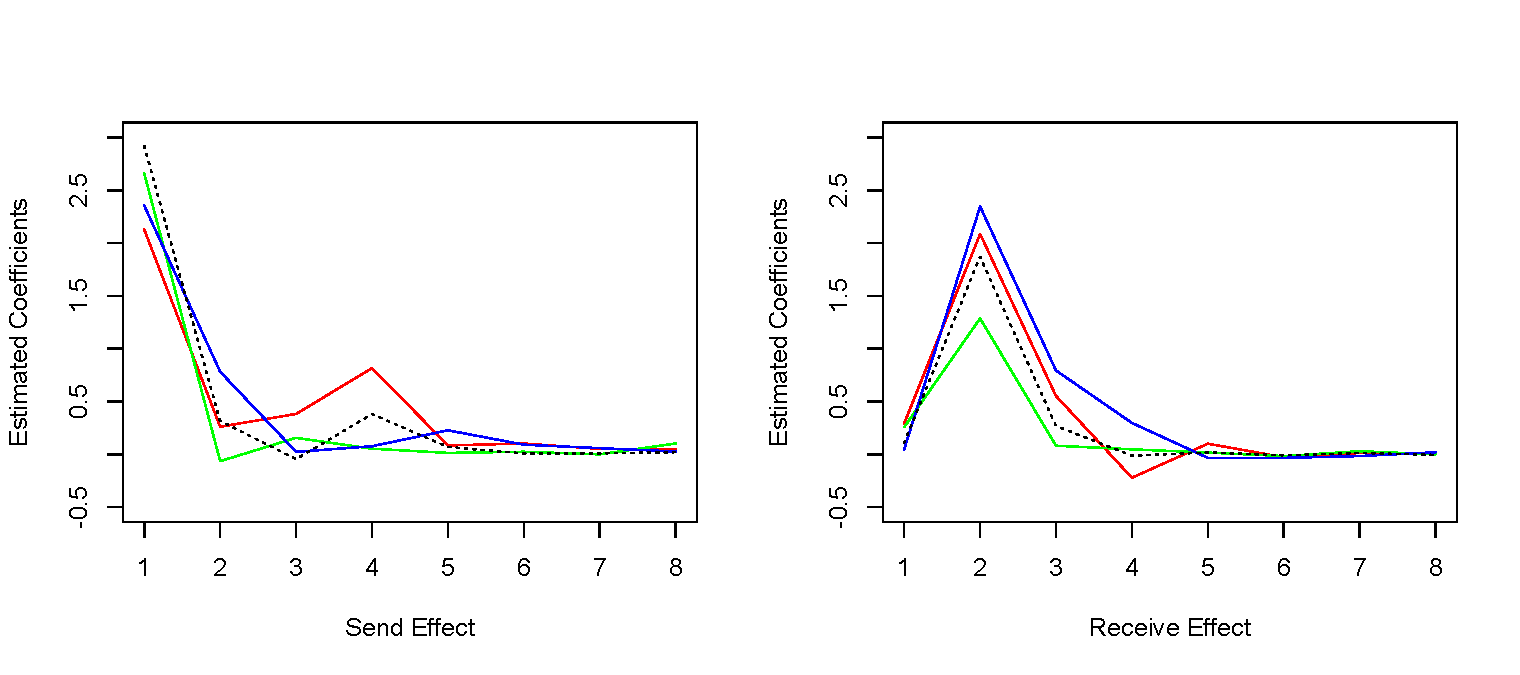
\includegraphics[width=1.1\textwidth]{Dareplot.pdf} 
	\caption{Comparison of Send (left) and Receive (right) effect based on periods in Table 1. (Red=Before, Green=During, Blue=After, and dot=Overall)}	\label{fig:Emailplo22t}
\end{figure}
\subsection{Lenoir County}
\footnotesize
\begin{table}[ht]
	\centering
	\begin{tabular}{ |c|ccc|c| } 
		\hline 
		\textbf{Period} &\textbf{Before Sandy} & \textbf{During Sandy} & \textbf{After Sandy} & \textbf{Overall} \\ 	\hline
		\textbf{\# emails}& 216 & 83 & 302 & 601 \\ 
		\hline
	\end{tabular}
	\caption{ Summary of Lenoir county email data based on time period}
	\label{table:nullDare22}
\end{table}
\normalsize
Before Sandy ranges from 2012-10-01 to 2012-10-21 (3 weeks), During Sandy ranges from 2012-10-22 to 2012-11-02 (2 weeks), and After Sandy ranges from 2012-11-03 to 2012-12-31 (8 weeks).
\footnotesize
\begin{figure}[ht]
	\centering
	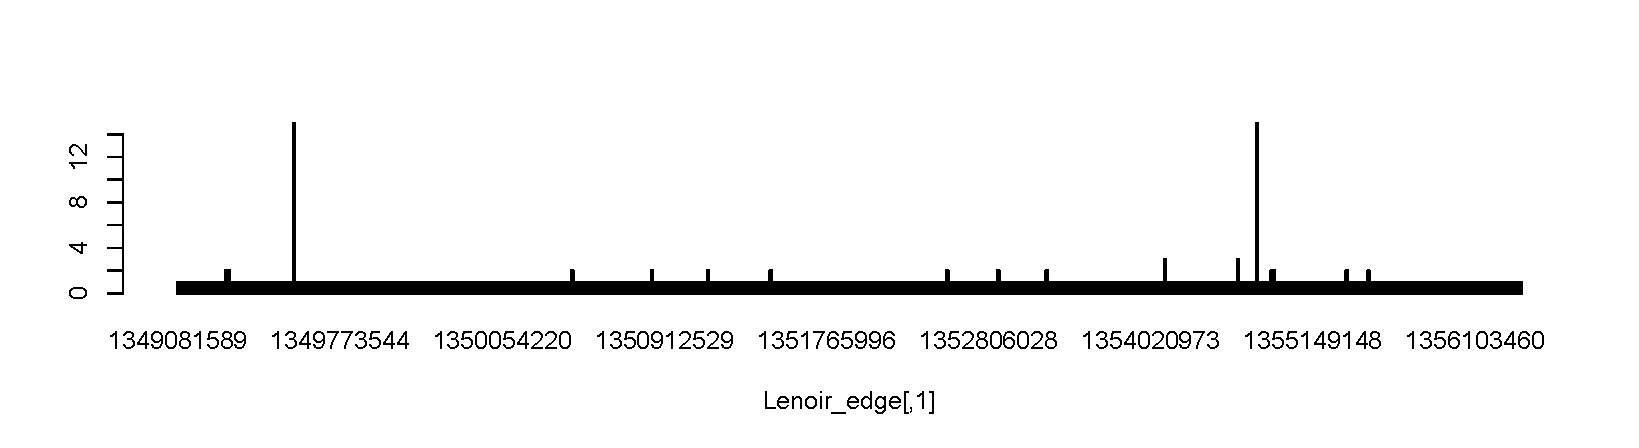
\includegraphics[width=1.1\textwidth]{LenoirEmails.pdf} 
	\caption{Frequency of Lenoir county emails from 2012-10-01 to 2012-12-31  }
	\label{fig:Emailplots32}
\end{figure}
\newpage
\subsection{Vance County}
\footnotesize
\footnotesize
\begin{table}[ht]
	\centering
	\begin{tabular}{ |c|ccc|c| } 
		\hline 
		\textbf{Period} &\textbf{Before Sandy} & \textbf{During Sandy} & \textbf{After Sandy} & \textbf{Overall} \\ 	\hline
		\textbf{\# emails}& 198& 18 & 55 & 271 \\ 
		\hline
	\end{tabular}
	\caption{ Summary of Vance county email data based on time period}
	\label{table:nullVance}
\end{table}
\normalsize
Before Sandy ranges from 2012-09-04 to 2012-10-21 (7 weeks), During Sandy ranges from 2012-10-22 to 2012-11-02 (2 weeks), and After Sandy ranges from 2012-11-03 to 2012-11-30  (4 weeks).
\footnotesize
\begin{figure}[ht]
	\centering
	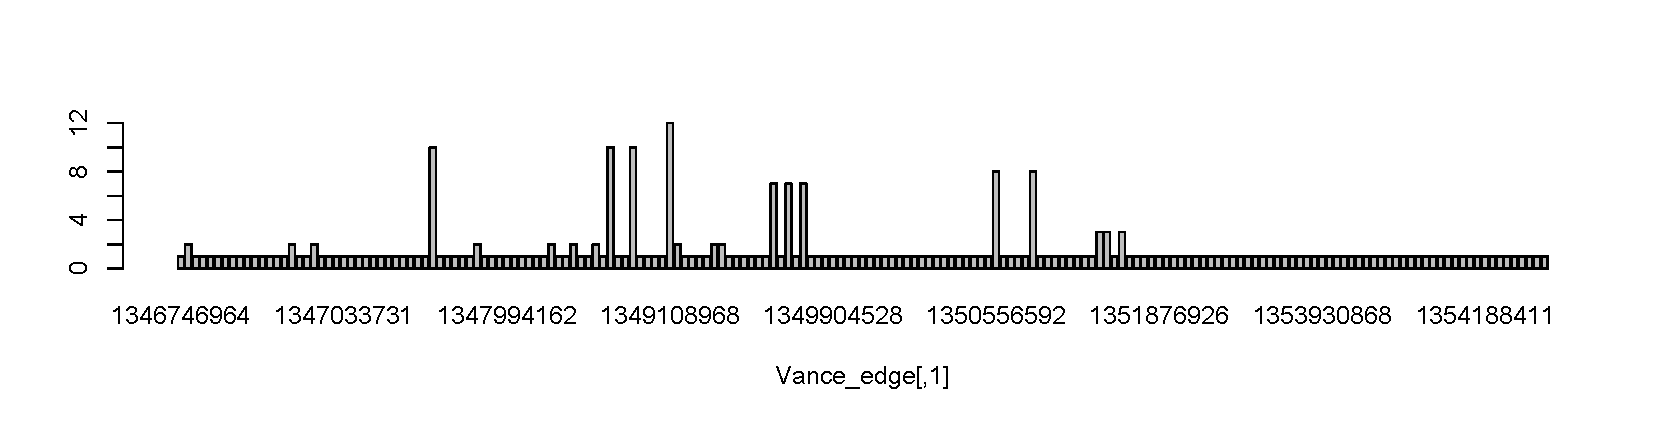
\includegraphics[width=1.1\textwidth]{VanceEmails.pdf} 
	\caption{Frequency of Vance county emails from 2012-09-04 to 2012-11-30  }
	\label{fig:Emailplots22}
\end{figure}
\end{document}